\begin{figure}
\centering
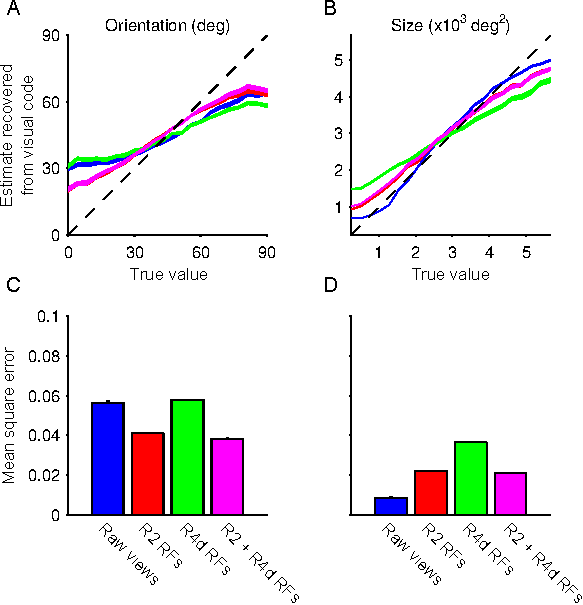
\includegraphics{figures/orsi}
\caption{How much shape information is preserved in the R2 population code?
Neural networks were trained to estimate the orientation and size of randomly generated 'blob' stimuli ($N=1000$) from different visual encodings (details same as for Figure~\ref{fig:elaz}).
A and B: Network performance in recovering stimulus orientation and size. Orientation was constrained between 0\degree\ and 90\degree, to avoid the problem of aliasing, and varied with 22 levels (conventions as in Figure~\ref{fig:elaz}).
C and D: Average network performance (Mean square error) for networks trained to recover orientation (C) or size (D) and for each type of visual input (colour code as previously). Standard error is shown, but is very small.
}
\label{fig:orsi}
\end{figure}
